\subsection{Foundation Laws}
\textbf{Physical Models -- Fitts' Law}:\\
Physical models can predict efficiency based on the physical aspects of a design. They calculate the time it takes to perform actions such as targeting a screen object and clicking on it.
Fitts' law can be used to determine the size and location of a screen object. It states that the time it takes to hit a target is a function of the size of the target and the distance to that target:

\begin{itemize}
\item Index of Difficulty (ID): Quantifies the difficulty of a (motor pointing) task based on width and distance
\begin{align*}
ID = \log_2(A / W+1)
\end{align*}
$A$=amplitude, $W$=width
\item Movement Time (MT): Quantifies the time it takes to complete a task based on the difficulty of the task (ID) and two empirically derived coefficients that are sensitive to the specific experimental conditions\\
\begin{align*}
MT = a + b \log_2(A / W+1) = a + b ID
\end{align*}(assuming linear movement speed).\footnote{Original form: $MT = a + b \log_2(2A / W)$}
$a \left[sec\right], b\left[sec/bits\right]$ constants dependent on the input device\\
$\rightarrow$ Fitts' law (1954) predicts that the time to acquire a target is in logarithmic relation the target size.\\
\begin{figure}[h!]
	\centering
	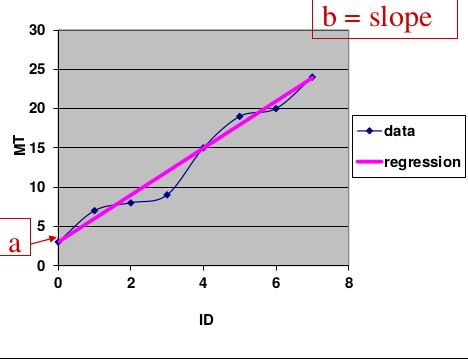
\includegraphics[width=.5\textwidth]{img/ch05_fitt.png}
	\caption{Linear Regression Model}
	\label{fitt}
\end{figure} 
\item Index of Performance (IP), also called throughput (TP): Based on the relationship between the time it takes to perform a task and the relative difficulty of the task
\end{itemize}
In practice $A$ corresponds to the distance from starting position, $W$ to the size of target along the line of motion. Common parameter values (e.g. for a mouse) are $a=50ms, b=150ms/bit$.
\begin{figure}[h!]
	\centering
	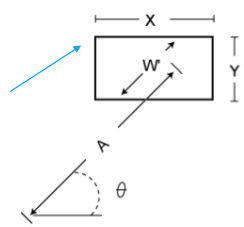
\includegraphics[width=.3\textwidth]{img/ch05_fitt1.png}
	\caption{Fitts' law in practice.}
	\label{fitt1}
\end{figure}
Fitt's Law is a predictive model of time to point at an object. Implications for interaction design in GUIs:
\begin{itemize}
\item Doubling the distance increases time but does not double it.
\item Increasing target size enables more rapid pointing.
\item MT for ``gross-movement tasks'': Formula from above, where $a$= time to start and stop in seconds for a device and $b$ = inherent speed of the device (e.g. a mouse)
\item Movement Time (MT) for ``precision pointing tasks'': $PPMT = a + b \log_2 (A/W + 1) + c log_2 (d/W)$, where $c$ = added constant, dependent on the user's context and $d$ = distance between hand location and spot where the user first touched the screen
\item GUIs with a Mouse Interface: 
\begin{itemize}
\item Overly elongated objects hold no advantage (W/H ratios of 3 and higher)
\item Objects should be elongated along the most common trajectory path (widgets normally approached from the side should use W, those approached from the bottom or top should use H).
\item Objects should not be offset from the screen edge
\item Fitts law does not address touch specific problems, e.g. fat finger
\end{itemize}
\item Fitts' Law is not 1:1 applicable to touch interfaces:
\begin{itemize}
\item Fat finger problem
\item Fingers are not moving directly from target to target but make a 3D movement
\item Fingers may directly reach target or need to be stretched or bended or a user may be even forced to change to 2-handed input
\item Screen size and hand size have a major impact on performance
\end{itemize}
\end{itemize} 
\textbf{Modelling Structure -- Hick's Law}:\\
Hick's Law states that the time $T$ needed to make a decision (e.g. a selection) is proportional to the log number of alternatives given.
\begin{align*}
T = b \cdot H
\end{align*}
where $H$ is the information-theoretic entropy of a decision:
\begin{align*}
H = 
\begin{cases}
\log_2(n+1), & n = \text{ alternatives of equal probability}\\
\sum p_i \log_2(\frac{1}{p_i + 1}), & p_i = \text{ probability of alternative }i
\end{cases}
\end{align*}
Note: Hick's Law does not apply if it requires linear search (e.g. a randomly ordered list of commands in a menu). It applies if the user can search by subdivision.\\
The total decision time in practice amounts to 
\begin{align*}
T = a + b \log_2(n+1)
\end{align*}
where $n$ is the number of choices. The coefficients are empirically determined from experimental design. Raskin (2000) suggests that $a= 50 ms$ and $b=150 ms/bit$ are sufficient place holders for ``back-of-the-envelope'' approximations.

\textbf{Power Law of Practice}:\\
Users get better every time they use a system. Neglecting disturbance and decay effects
\begin{align*}
Time = B\cdot N^{-\alpha}
\end{align*}
where $N$ = Trial Number, $B, \alpha$ = constants

\subsection{Applied Design Guidelines \& Principles: Mental Models -- Mapping -- Affordances}
\textbf{Mental Models}: \\
People use a mental model to have a basic understanding of what is going on. The mental model is often unsharp, e.g. you know your car speeds up when pressing the gas pedal, but the concept behind is unsharp. Unsharp models might be sufficient, but in certain situations they might not be enough to explain the system. Interaction that is both predictive and explanatory can be understood with the concept of mental models. Mental models are
\begin{itemize}
\item Unscientific: they are based on guesswork
\item Partial: They do not describe the whole system
\item Unstable: They evolve an adapt to context and experience
\item Inconsistent: Some parts of the model may be incompatible with other parts of the system
\item Personal: They are specific to individuals
\end{itemize}
However, they can be used to foster understanding and building a correct model and thus increase usability. E.g. Error Avoidance Design Guidelines exploit natural mappings between intentions and possible actions, between actions and their effects on the system state and what is perceivable, as well as between the system state and the needs, intentions and expectations of the user.\\

\textbf{Principles of Good Design (Don Norman)}:\\
An interface should include good mappings that show the relationship between stages. There should be a clear correlation between control element and action. A ``good'' mapping should be understandable, consistent, recognizable or quickly learnable and natural (consistent to the user's knowledge, world and domain knowledge). For example for cooking plates it would be helpful to arrange the buttons corresponding to the plates exactly like the plates themselves.\\ \\

\textbf{Constraints} lead humans to build correct mental models. They guide the user to the next appropriate action or decision and also minimize the chance to make errors.
\begin{itemize}
\item physical constraints (dial vs. button)
\item semantic constraints (assumption that create something meaningful)
\item cultural constraints (borders provided by cultural conventions, e.g. traffic signs, colours, ..)
\item logical constraints (restrictions due to reasoning)
\end{itemize}
It is good (for safety) to add some redundancy, as constraints can only work at their own level (e.g. having plugs color- and shape-coded in safety-critical situation).\\

\textbf{Affordances (Gibson)}:\\
To build a mental concept of a system we need to interpret symbols and components. This can be seen as the functionality of the device and what we actually want to do\\
$\rightarrow$ Semantic and Articulator Distance\\
Don Norman developed this concept further picking up the idea of affordances. It refers to the perceived and actual properties of an (everyday) object, which have to be matched:\\
-- Make usable properties visible\\
-- Use natural associations\\
-- Give Feedback\\
Objects and environments imply their usage through Gestalt, e.g. door handle animates to press, cup to drink $\rightarrow$ Partially learned!\\
\textbf{Normans Evaluation/Execution Action Cycle}:
\begin{figure}[h!]
	\centering
	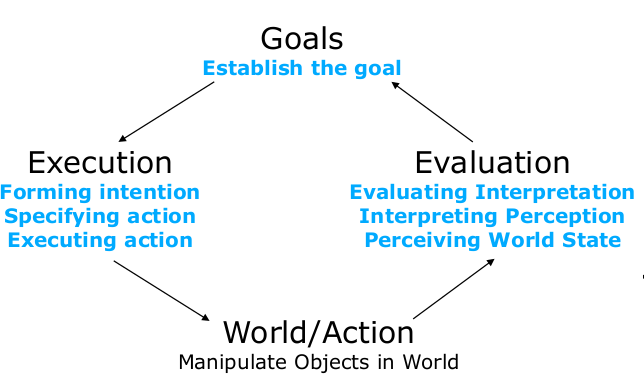
\includegraphics[width=.4\textwidth]{img/ch05_cycle1.png}
	\caption{Evaluation/Execution Action Cycle}
	\label{cy}
\end{figure}
\begin{itemize}
\item Gulf of execution: Mismatch between the user's intentions and the allowable actions. Problems:
\begin{itemize}
\item Forming intention $\rightarrow$ Insufficient knowledge of concept
\item Specifying action $\rightarrow$ Insufficient knowledge of usage
\item Executing action $\rightarrow$ Difficult access to function
\end{itemize}
The difference between the intentions and the allowable actions is the Gulf of Execution. How directly can the actions be accomplished? Do the actions that can be taken in the system match the actions intended by the person?\\
$\rightarrow$ Good design minimizes the Gulf of Execution
\item Gulf of evaluation: Mismatch between the system's representation and the users' expectations. Problems:
\begin{itemize}
\item Evaluating Interpretation $\rightarrow$  Comparing goal and state
\item Interpreting Perception $\rightarrow$ Interpretation of state
\item Perceiving World State $\rightarrow$ perception of State
\end{itemize}
You may check how easy you are able to determine the function, determine what actions are possible, determine mapping from intention to physical movement, perform the action, determine whether the system in the desired state, determine mapping from system state to interpretation and determine what state the system is in. The Gulf of Evaluation reflects the amount of effort needed to interpret the state of the system and how well this can be compared to the intentions. Is the information about state of the system easily accessible? Is it represented to ease matching with intensions?\\
$\rightarrow$ Good design minimizes the Gulf of Evaluation
\end{itemize}

Example: The user wants a document written on the system in paper (the goal).\\
Gulf of Execution: What actions are permitted by the system to achieve this goal?\\
Gulf of Evaluation: Is the process observable? Are intermediate steps visible?\\
Implications on design:
\begin{itemize}
\item Principles of good design (Norman):
\begin{itemize}
\item Stage and action alternatives should be always visible
\item Good conceptual model with a consistent system image
\item Interface should include good mappings that show the relationship between stages
\item Continuous feedback to the user
\end{itemize}
\item Critical points/failures:
\begin{itemize}
\item Inadequate goal formed by the user
\item User does not find the correct interface / interaction object
\item User many not be able to specify / execute the desired action
\item Inappropriate / mismatching feedback
\end{itemize}
\end{itemize}

\subsection{Task Analysis}
A \textbf{goal} is a state of the application domain that a work system wishes to achieve. Goals are specified at particular levels of abstraction. \\
A \textbf{task} is a goal together with some ordered set of actions. Or more elaborated:
A task is a structured set of activities required, used or believed to be necessary by an agent to achieve a goal using a particular technology. A task will often consist of subtasks where a subtask is a task at a more detailed level of abstraction. The structure of an activity may include selecting between alternative actions, performing some actions a number of times and sequencing of actions.\\
An action is a task which has no problem solving associated with it and which does not include any control structure. Actions and task will be different for different people.
\textbf{Task analysis} is the study of how work is achieved by tasks. It is about understanding people and how they carry out their work (part of human-centred design):
\begin{itemize}
\item identify a set of methods people use to carry out their work
\item identify if they reach the goal
\item calculate how long it takes to reach the goal
\end{itemize}
Two main categories of task analysis methods concerned with the logic of tasks (sequence of steps to achieve a goal) and the cognitive\footnote{Cognition: thinking, solving problems, learning, memory $\rightarrow$ HIP!\\ Representations of things that people are assumed to have in their heads $\rightarrow$ mental models} aspects (understanding which cognitive processes the work system will have to undertake to achieve a goal).\\
Different Task Analysis methods can be sorted into four \textbf{dimensions}: notation, usability for communication, usability for modelling tasks, adaptability to new types of systems/aims/requirements. Task analysis is an integral part of System Development and undertaken several times, during analysis (independent from technology, understanding the ``essentials'', current way of doing things), design (cognitive load minimization) and evaluation (dependent on technology, degree of achievement of work).\\ \\
In the following, two models will be discussed: Hierarchical Task Analysis (HTA), concerned with the logic of the task, and Goal-based Task Analysis (GOMS), concerned with the cognitive analysis of the task. Both models rely on Cognitive System models (see previous chapters).\\ \\ 
\textbf{Hierarchical Task Analysis (HTA)}: 
Graphical representation of a task structure in structure chart notation: sequence of tasks, subtasks and actions as hierarchy, actions can be repeated (iteration), alternative actions possible (selection), annotations to indicate plans (optional). This is not trivial: acquisition of task and subtask descriptions, hierarchical modelling, iterative process.
\begin{figure}[h!]
	\centering
	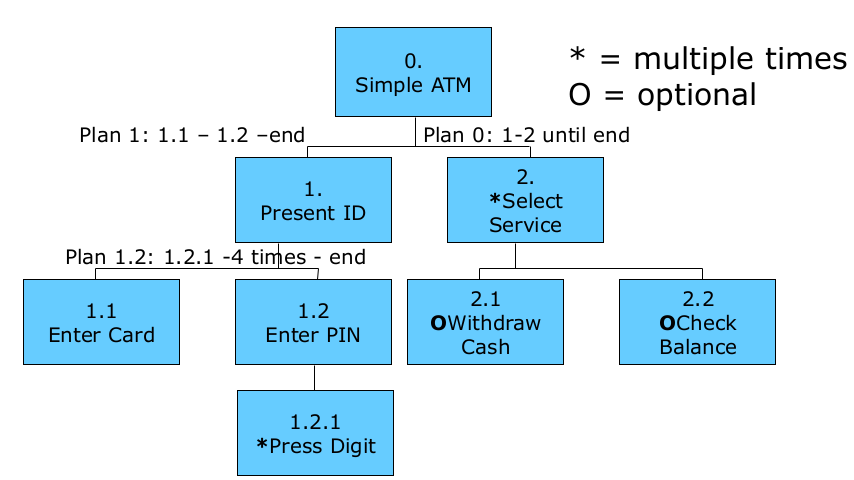
\includegraphics[width=.5\textwidth]{img/ch05_hta.png}
	\caption{HTA -- Example}
	\label{hta}
\end{figure}

\textbf{Goal-based Task Analysis -- GOMS}: Goals, Operators, Methods, Selection Rules\\
An application of Human Information Processing and Task Analysis/Decomposition focusing on Cognitive Load Analysis. Introduced by Card, Moran \& Newell (1983) they feature an explicit task structure:
\begin{itemize}
\item Hierarchy of goals and sub-goals
\item Procedure: define goals and refine them
\item Outcome are several sheets of GOMS descriptions, starting with the topmost description
\item Methods in the topmost description are subsequently refined in the ``lower'' GOMS descriptions
\end{itemize}
CNM-GOMS -- Engineering model of user interaction:
\begin{itemize}
\item Goals -- user's intentions (tasks): e.g. write a text, something the user perceives as a task
\item Operators -- actions to complete task: Basic, low level action to perform or basic mental state; cognitive, perceptual \& motor (HIP); e.g. press X, read dialog; time of activity can be given
\item Methods (Subgoals) -- sequences of actions (operators): may be multiple methods for accomplishing same goal, e.g. shortcut key or menu selection
\item Selections -- rules for choosing appropriate method: method predicted based on context; selection rules are separately described
\end{itemize}
CPM-GOMS represent Cognitive, Perceptual, Motor operators. It uses Program Evaluation Review Technique (PERT) charts which map task durations using the critical path method (CPM). It is based directly on the Model Human Processor which assumes that perceptual, cognitive, and motor processors function in parallel.
\begin{figure}[h!]
	\centering
	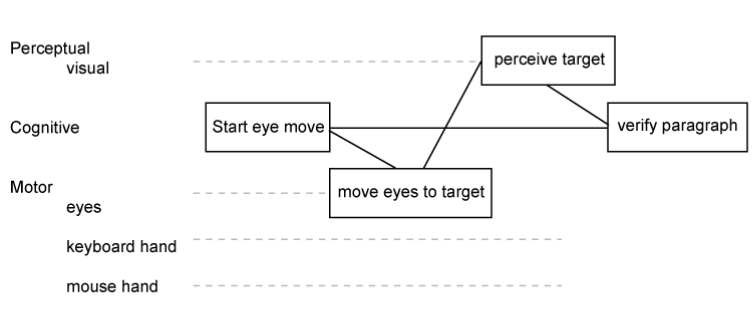
\includegraphics[width=.5\textwidth]{img/ch05_pert.png}
	\caption{PERT chart -- Example}
	\label{pert}
\end{figure}

\textbf{Keystroke Level Model (KLM)}: The KLM is a practical design tool that can capture and calculate the physical actions a user will have to carry out to complete specific tasks. It can be used to determine the most efficient method and its suitability for specific contexts. 
\begin{itemize}
\item Given:
\begin{itemize}
\item A task (possibly involving several subtasks)
\item The command language of a system
\item The motor skill parameter of the user
\item The response time parameters
\end{itemize}
\item Predict: The time an expert user will take to execute the task using the system, provided that he or she uses the method without error.
\end{itemize}
The KLM is comprised of Operators, Encoding methods, and Heuristics for the placement of mental (M) operators. Operators include \textit{Press a key or button} (K), \textit{Point with mouse} (P), \textit{Home hands to keyboard or peripheral device} (H), \textit{Draw line segments} (D), \textit{Mental preparation} (M), \textit{System response} (R)